\documentclass{article}[12pt]
\usepackage{verbatim}
\usepackage{fullpage}
\usepackage{graphicx}

\title{CS246 Assignment 4}
\author{Nissan Pow}

\begin{document}
\maketitle

\section*{Question 1}
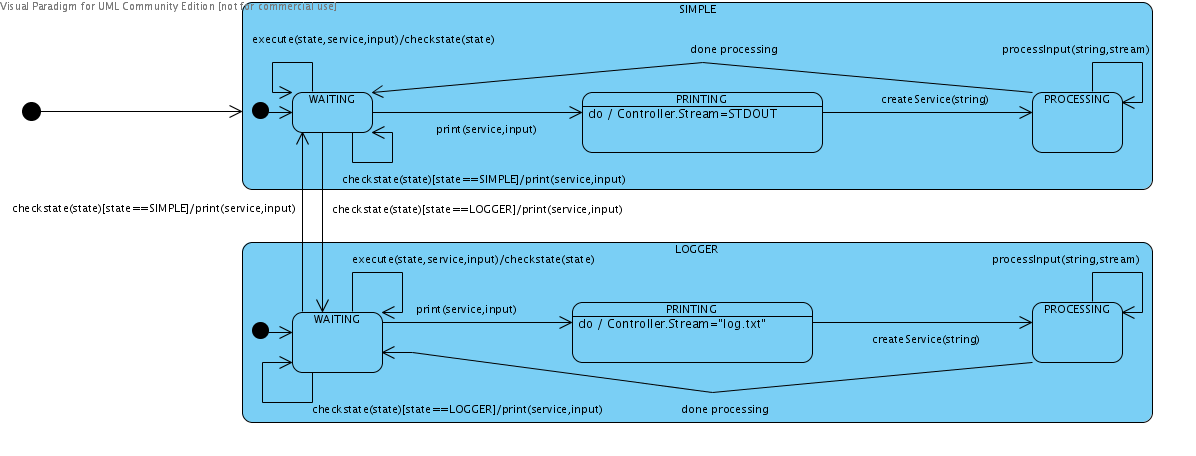
\includegraphics[scale=0.45]{cs246_a4q1.png}

\section*{Question 2}
\begin{itemize}
  \item Singleton \\
    Classes: Controller, SortService, StorageService \\
    Fuctions: Controller::getInstance(), SortService::getInstance(), StorageService::getInstance() \\
    Description: getInstance() ensures that there is only one instance of Controller, SortService, and StorageService \\

  \item State \\
    Classes: ControllerState, LoggerState, SimpleState \\
    Functions: ControllerState::print(string,string), ControllerState::checkState(string), LoggerState::print(string,string), LoggerState::checkState(string),
    SimpleState::print(string,string), SimpleState::checkState(string) \\
    Description: ControllerState is an interface for encapsulating the behaviour associated with the two different states, Simple and Logger. \\
    
  \item Factory Method \\
    Classes: Service, SortService, StorageService \\
    Functions: Service::createService(string) \\
    Description: Service::createService(string) encapsulates the knowledge of which service (sort or storage) to create and delegates
    the creation of the services to its subclasses.
    
  \item Template Method \\
    Classes: Service, SortService, StorageService \\
    Functions: Service::routine(), SortService::routine(), StorageService::routine() \\
    Description: The routine() method is inherited and implemented by both of the subclasses. Thus a different routine() algorithm
    can be performed in each of the subclasses, while keeping the general algorithm for Service::processInput() and Service::parseInput() the same.


\end{itemize}


\section*{Question 3}
The Strategy pattern could be applied instead of using Template Methods. We could make Service an abstract class, and then implement
different Service algorithms in each of its subclasses. 

\section*{Question 5}
This is not recommended since there is a tight coupling between the LoggerState and the IOStream classes, so that if we decide
to change IOSream, we would also have to change LoggerState. We can decouple these 2 classes by implementing the Adapter Pattern,
so that the Adapter handles requests transparently with the IOStream. Using the Adapter Pattern, we can easily include a FileStream
class. Then MyStream::print() will call the appropriate print method (IOStream::print() or FileStream::print()) as necessary.

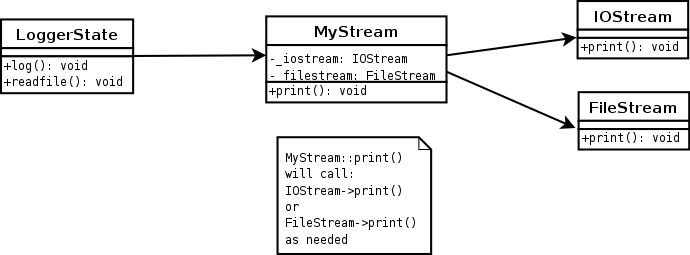
\includegraphics[scale=0.45]{a4q5.png}

\end{document}

